\documentclass[twocolumn,showpacs,floatfix,nofootinbib,longbibliography]{revtex4-1}
\usepackage{graphicx}
\usepackage{bm} % bold math
\usepackage{amssymb} % use this package to enable \nrightarrow command
\usepackage{amsmath} % use this package to enable \xrightarrow command
\usepackage{braket} % use for Dirac bra-kets : \rangle \labgle & \mid
\usepackage{natbib} % bibtex package
\usepackage{hyperref}


\begin{document}

\title{Skyrmion-induced localized state in a two-dimensional superconductor}

\author{Sho Nakosai$^{1,2}$}
\author{Sergey S. Pershoguba$^{1}$}
\author{Alexander V. Balatsky$^{1,3}$}
\affiliation{$^1$Nordita, Center for Quantum Materials, KTH Royal Institute of Technology, and Stockholm University, Roslagstullsbacken 23, S-106 91 Stockholm, Sweden}
\affiliation{$^2$Department of Applied Physics, University of Tokyo, Tokyo 113-8656, Japan}
\affiliation{$^3$Institute for Materials Science, Los Alamos National Laboratory, Los Alamos, NM 87545, USA}

\date{\today}


\begin{abstract}
Skyrmions are nice
\end{abstract}

\pacs{ }   

%%%%%%%%%%%%%%%%%%%%%%%%%%%%%%%%%%%%%%%%%%%%%%%%%%%%%%%%%%%%%%%%%%%%%%%%%%

\maketitle
%%%%%%%%%%%%%%%%%%%%%%%%%%%%%%%%%%%%%%%%%%%%%%%%%%%%%%%%%%%%%%%%%%%%%%%%%%%
\paragraph*{Introduction.} \label{sec:intro}
%%%%%%%%%%%%%%%%%%%%%%%%%%%%%%%%%%%%%%%%%%%%%%%%%%%%%%%%%%%%%%%%%%%%%%%%%%%

General context of skyrmions asd tolopolical excitations: memory, manipulation, local creation via SP STM.
Extension of skyrmion discussion to the case of hybrid structures: SC and Skyrmion. What are the consequenc of brining topological exchange field into SC. Question we address is the possible local spectroscopic signatures of SC quasiparticles in SC due to skyrmion field. We know from the past discussion that there are impurity bound states in SC near magnetic impurities. We have now the framework to address formation of bound states. Talk about local single impurity limit (YSR) and show the cartoon of the local and extended skyrmion and spectra. There are two effects: local scattering and Zeeman field hence the DOS will be split etc.  Draw similarities and differences with single imp.
In parallel with skyrmion discovery the local imaging using magnetic probes like MFM and SP-STM allowed one to image the matter at atomic resolution while also resolving spin content of electron carriers in the substrate.  
Here we prove the existence of the new type of localized excitation on the skyrmion core we call  Sc-YSR state (alternative is skyrmion bound state (sbs)).  Show the main results upfront in the introduction. Both LDOS and SP-LDOS. 
Main section: 

Introduce T matrix and results for analytic solution.  
Introduce the numerical approach and presenst the results oas a function of position and as a function of energy. Kind of same figs as in Sho’s talk. 
Discuss the results and what it means, how big the signal is etc. Unfortunately we do not see any topological state at zero energy and as such these result represent a new kind of magnetic texture induced states that exhibit intragap states.



%%%%%%%%%%%%%%%%%%%%%%%%%%%%%%%%%%%%%%%%%%%%%%%%%%%%%%%%%%%%%%%%%%%%%%%%%%%
\paragraph*{Skyrmions in ferromagnetic films. [Comment: here we discuss skyrmions in ferromagnets. Define topological numbers and moments of skyrmions fields.]} \label{sec:skyrmion}
%%%%%%%%%%%%%%%%%%%%%%%%%%%%%%%%%%%%%%%%%%%%%%%%%%%%%%%%%%%%%%%%%%%%%%%%%%

%%%%%%%%%%%%%%%%%%%%%%%%%%%%%%%%%%%%%%%%%%%%%%%%%%%%%%%%%%%%%%%%%%%%%%%%%%%
\begin{figure} \centering
(a) 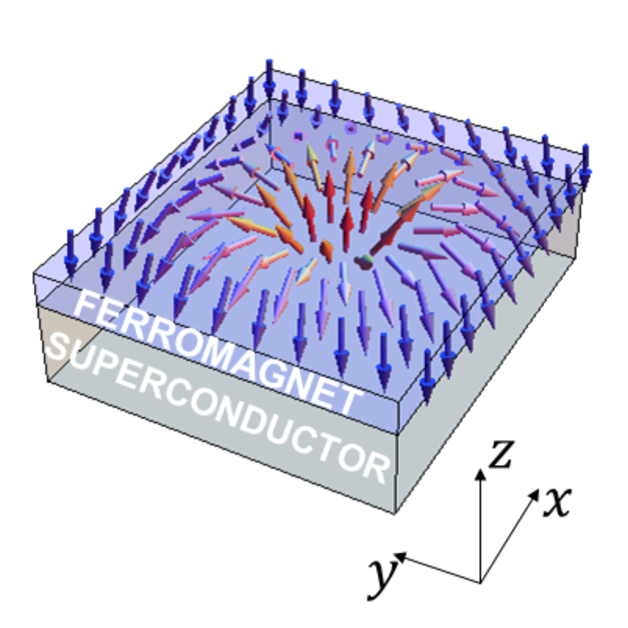
\includegraphics[width=0.4\linewidth]{SkyrmA}  
(b) 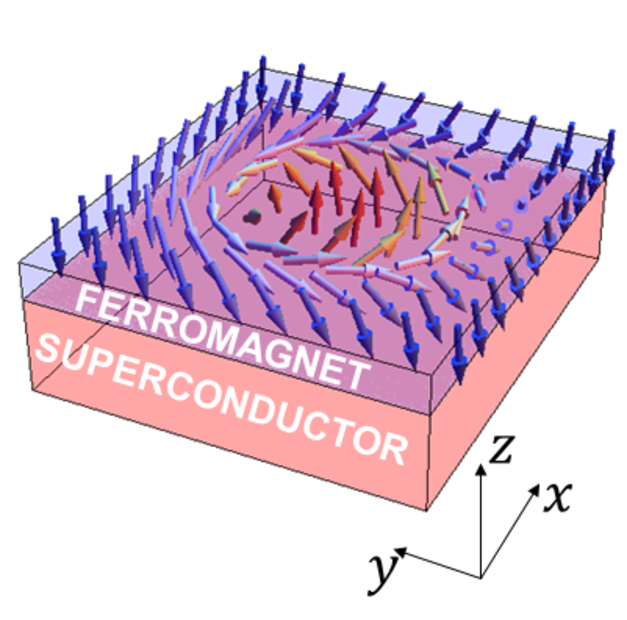
\includegraphics[width=0.4\linewidth]{SkyrmB} 
\caption{(Color online.) Ferrormagnetic film deposited on top of a superconductor. The ferromagnetic vector has skyrmion configuration. (a) Monopole skyrmion.  (b) Anapole skyrmion. } \label{fig:skyrmion}
\end{figure}
%%%%%%%%%%%%%%%%%%%%%%%%%%%%%%%%%%%%%%%%%%%%%%%%%%%%%%%%%%%%%%%%%%%%%%%%%%




Let the three-dimensional vector $S(\bm r) = (S_x,S_y,S_z)$ describe the configuration of the ferromagnetic vector in a two-dimensional ferromagnetic film $\bm r = (x,y)$. The configurations of the field $S(\bm r)$ shown in Fig. \ref{fig:skyrmion}(a) and (b) are referred to as skyrmions. The skyrmion configuration of the field is characterized by the topological charge 

\begin{align}
	Q = \frac{1}{4\pi} \int d^2r \, \hat {\bm S}\cdot (\nabla_x\hat {\bm S}\times\nabla_y\hat {\bm S}), \quad \hat {\bm S}= \frac{\bm S}{S}, 
	\label{topCharge}
\end{align}
which cannot be altered by the continuous transfomation of the field.  We also characterize the skyrmion fields by the zeroth and first moments
\begin{align}
	S^{(0)}_i = \int  d^2r \, \left[S_i(\bm r)-S_i(\infty)\right],\,\, i\in \{x,y,z\}, \label{S0} \\
	S^{(1)}_{ij} = \int  d^2r \, \left[S_i(\bm r)-S_i(\infty)\right] r_j,\,\, j\in \{x,y\}. \label{S1}
\end{align}
The zeroth moment $\bm S^{(0)} = S_{\rm eff} \hat{\bm z}$ characterizes the effective out-of-plane magnetic moment of the skyrmion and is equal for the two skyrmions shown in Fig.~{\ref{fig:skyrmion}}(a) and (b). Whereas, the first-order moment $S^{(1)}_{ij}$ characterizes the in-plane pattern of the ferromagnetic vector $\bm S(\bm r)$. Note that for the cylindrically symmetric field $S(\bm r)$, the first order moment defined in Eq.~(\ref{S1}) can be expanded in the symmetric and antisymmetric parts $S^{(1)}_{ij}=S_{\rm mono}\,\delta_{ij} + S_{\rm ana}\,\epsilon_{ijz}$. The skyrmions shown in Fig.~\ref{fig:skyrmion}(a) and (b) have monopole $S_{\rm mono}$ and anapole $S_{\rm ana}$ moments correspondingly, hence the name of the skyrmions. However the two types of the skyrmions have the same topological charge~(\ref{topCharge}) and thus can be continuosly deformed into each other. 

%%%%%%%%%%%%%%%%%%%%%%%%%%%%%%%%%%%%%%%%%%%%%%%%%%%%%%%%%%%%%%%%%%%%%%%%%%%
\paragraph*{Model. [Comment: here we introduce the model of coupling between the FM film and BCS superconductor.]} \label{sec:model}
%%%%%%%%%%%%%%%%%%%%%%%%%%%%%%%%%%%%%%%%%%%%%%%%%%%%%%%%%%%%%%%%%%%%%%%%%%
The model is given by the following Hamiltonian 
\begin{align}
	\mathcal H &= \frac{1}{2}\int d^2r\, \Psi^\dagger(\bm r)\left[\xi(\bm p)\tau_z+\Delta \tau_x - \bm S(\bm r)\cdot\bm\sigma\right]\Psi(\bm r), \label{ham} \\
  & \xi(\bm p) = \frac{p^2}{2m}-\mu,\quad \bm p = -i(\nabla_x,\nabla_y),
\end{align}
which describes the proximity coupling of the ferromagnetic vector $S(\bm r)$ to the itinerant electrons of a two-dimensional (2D) superconductor with the superconducting gap $\Delta$. The Pauli matrices $\bm \tau$ and $\bm \sigma$ act, respectively, in the particle-hole and spin subspaces of the four-component spinor $\Psi = (\psi_\uparrow,\psi_\downarrow,\psi^\dagger_\downarrow,-\psi^\dagger_\uparrow)^T$.
%%%%%%%%%%%%%%%%%%%%%%%%%%%%%%%%%%%%%%%%%%%%%%%%%%%%%%%%%%%%%%%%%%%%%%%%%%%
\paragraph*{T-matrix analysis} \label{sec:analytics}
%%%%%%%%%%%%%%%%%%%%%%%%%%%%%%%%%%%%%%%%%%%%%%%%%%%%%%%%%%%%%%%%%%%%%%%%%%%
Superconductor-ferromagnet heterostructures were recently proposed as a viable platform for realizing topological superconductivity (TS) \cite{Lutchyn2010,Oreg2010, Sau2010}, which can host Majorana fermion quasiparticles at vortex cores and boundaries \cite{Kitaev2001, Alicea, Beenakker2013}. Majorana fermions obey non-Abelian statistics and may be utilized for topological quantum computation \cite{Read2000, Ivanov2001, Nayak2008}.  The key ingredients driving these systems in the topologically non-trivial regime are the spin-orbit coupling (SOC) and magnetism. Recently, the search for experimental realizations of TS has also led to engineering the impurity bands of the Yu-Shiba-Rusinov (YSR) states \cite{Yu,Shiba,Rusinov}, induced by magnetic atoms on the surface of a superconductor \cite{Choy2011, Nadj-Perge2013, Klinovaja2013, Vazifeh2013, Braunecker2013, Pientka2013, Nakosai2013, Poyhonen2014, Reis2014, Brydon2015, Rontynen2014, Li2015}. Following this recipe, zero-energy peaks in the tunneling spectrum were recently measured at the ends of a one-dimensional (1D) chain of magnetic atoms \cite{Yazdani2014}. Such a tunneling spectrum could be the evidence of Majorana edge states, although alternative explanations are also possible \cite{Sau2015}.




\begin{equation}
 T = \frac{V}{1-vg_{00}}
\end{equation}

%%%%%%%%%%%%%%%%%%%%%%%%%%%%%%%%%%%%%%%%%%%%%%%%%%%%%%%%%%%%%%%%%%%%%%%%%%%
\paragraph*{Numerical analysis.} \label{sec:numerics} 
%%%%%%%%%%%%%%%%%%%%%%%%%%%%%%%%%%%%%%%%%%%%%%%%%%%%%%%%%%%%%%%%%%%%%%%%%%%

%%%%%%%%%%%%%%%%%%%%%%%%%%%%%%%%%%%%%%%%%%%%%%%%%%%%%%%%%%%%%%%%%%%%%%%%%%%
\paragraph*{Discussion [Comment: here we discuss importance. Long-range interactions between skyrmions mediated by superconductivity. ] } \label{sec:discussion} 
%%%%%%%%%%%%%%%%%%%%%%%%%%%%%%%%%%%%%%%%%%%%%%%%%%%%%%%%%%%%%%%%%%%%%%%%%%%



%%%%%%%%%%%%%%%%%%%%%%%%%%%%%%%%%%%%%%%%%%%%%%%%%%%%%%%%%%%%%%%%%%%%%%%%%%%
\paragraph*{Conclusion} \label{sec:conclusion}
%%%%%%%%%%%%%%%%%%%%%%%%%%%%%%%%%%%%%%%%%%%%%%%%%%%%%%%%%%%%%%%%%%%%%%%%%%%




\newpage
%%%%%%%%%%%%%%%%%%%%%%%%%%%%%%%%%%%%%%%%%%%%%%%%%%%%%%%%%%%%%%%%%%%%%%%%%%%%%
%\bibliographystyle{apsrev4-1}
\bibliography{Skyrmion}
%%%%%%%%%%%%%%%%%%%%%%%%%%%%%%%%%%%%%%%%%%%%%%%%%%%%%%%%%%%%%%%%%%%%%%%%%%%%%


\appendix 

%%%%%%%%%%%%%%%%%%%%%%%%%%%%%%%%%%%%%%%%%%%%%%%%%%%%%%%%%%%%%%%%%%%%%%%%%%%%%
\section{T-matrix analysis} \label{sec:appendixTMatrix}
%%%%%%%%%%%%%%%%%%%%%%%%%%%%%%%%%%%%%%%%%%%%%%%%%%%%%%%%%%%%%%%%%%%%%%%%%%%%%
In this section, we give an analytic treatment of the skyrmion-induced bound states using the T-matrix approximation. Starting from the Hamiltonian (\ref{ham}) in the second-quantized form, we write the Bogolyubov-de Gennes (BdG) Hamiltonian as 
\begin{align}
	& H_{\rm BdG} = H(\bm p) + V(\bm r),\quad {\rm where} \nonumber \\
& H(\bm p) = \xi(\bm p)\tau_z+\Delta \tau_x - \bm S(\infty)\cdot\bm\sigma,\quad \bm S(\infty) = -S\,\hat{\bm z}, \nonumber\\
& V(\bm r) = -\left[ \bm S(\bm r)-\bm S(\infty)\right]\cdot\bm\sigma \label{v0}
\end{align}
The momentum-dependent part $H(\bm p)$ describes a superconductor coupled to a spatially uniform ferromagnetic vector $\bm S(\infty)$, whereas the position-dependent piece $V(\bm r)$ describes the local perturbation due to the skyrmion. Physically, the superconducting coherence legth $\xi\sim 100$\,nm is much greater than the radius of the skyrmion $R\sim 10$\,nm (plug the real numbers from Wiesendanger papers), i.e. $\xi\gg R$. Therefore, the superconductivity does not ``resolve'' the fine details of the skyrmionic configuration of the field  $\bm S(\bm r)$, but rather ``sees'' its long-wavelength characteristics such as the moments described by Eqs.~(\ref{S0}) and (\ref{S1}). Motivated by this logic, we substitute the original skyrmionic field $\bm S(\bm r)$ by its local version 
\begin{equation}
	\bm S(\bm r) - \bm S(\infty) = \left[ S_{\rm eff}\, \hat{\bm z} - S_{\rm mono}\, \bm \nabla\right] \delta^2(\bm r).
	\label{S}
\end{equation}
By plugging Eq.~(\ref{S}) in the equations for the moments~(\ref{S0}) and (\ref{S1}), one can verify the definitions of the effective $S_{\rm eff}$ and monopole $S_{\rm mono}$ moments.  The latter simplified field $\bm S(\bm r)$ is especially convenient for the T-matrix calculation, which we now proceed to. We take into account (\ref{S}) and calculate the Fourier transform of Eq.~(\ref{v0})  
\begin{equation}
	V(\bm p) = -S_{\rm eff}\,\sigma_z +  i \,S_{\rm mono} \, \bm \sigma\cdot \bm  p,
	\label{vp}
\end{equation}
using which we write an intergal equation for the T-matrix
\begin{align}
	T\left(\bm p^{out},\bm p^{in}\right) &= V \left(\bm p^{out}-\bm p^{in}\right) \nonumber \\
	& + \int \frac{d^2p'}{(2\pi)^2} V\left(\bm p^{out}-\bm p'\right) G(\omega,\bm p')  T\left(\bm p',\bm p^{in}\right).
	\label{integEq}
\end{align}
Here, the bare Green's function of the superconductor is defined as 
\begin{align}
	G(\omega,\bm p) = \frac{1}{\omega-H(\bm p)} = \frac{1}{\omega-\xi(\bm p)\tau_z-\Delta \tau_x - S\sigma_z}.
\end{align}
Since in the case of the superconductivity we are interested in the scatterings close to the Fermi surface, we use $\bm p^{out} = p_F\, \bm n^{out}$ and $\bm p^{in} = p_F \,\bm n^{in}$, where the in-plane unit vectors $\bm n^{out}$ and $\bm n^{in}$ determine the direction of scattering on the Fermi surface.  Then, we seek the T-matrix in the following form
\begin{align}
	T\left(\bm n^{out},\bm n^{in}\right) &= A + B_i n^{\rm out}_i + C_i n^{\rm in} + D_{ij} n^{\rm out}_i n^{\rm in}_j, \label{ansatz}
\end{align}
where  $A,B_i,C_i$ and $D_{ij}$ are the matrices in the four-components space $\sigma\otimes\tau$. We substitute ansatz~(\ref{ansatz}) in the integral Eq.~(\ref{integEq}) and find the T-matrix
\begin{widetext}
\begin{equation}
	T\left(\bm n^{out},\bm n^{in}\right) = \frac{-S_{\rm eff}\sigma_z+i\,S_{mono}\, \bar G_{00}\, p_F \,\bm \sigma\cdot(\bm n^{\rm out+}- \bm n^{\rm in}) +S^2_{mono}\, \bar G_{00}\, p^2_F \,\left(\bm \sigma\cdot\bm n^{\rm out}\right)\,\left(\bm \sigma\cdot \bm n^{\rm in}\right)}{1+S_{\rm eff}\sigma_zG_{00}-S^2_{\rm mono}p_F^2G_{00}\bar G_{00}}
\end{equation}
\end{widetext}
Define $G_{00}$. 
%%%%%%%%%%%%%%%%%%%%%%%%%%%%%%%%%%%%%%%%%%%%%%%%%%%%%%%%%%%%%%%%%%%%%%%%%%%%%
\subsection{LDOS} \label{sec:LDOS}
%%%%%%%%%%%%%%%%%%%%%%%%%%%%%%%%%%%%%%%%%%%%%%%%%%%%%%%%%%%%%%%%%%%%%%%%%%%%%
%%%%%%%%%%%%%%%%%%%%%%%%%%%%%%%%%%%%%%%%%%%%%%%%%%%%%%%%%%%%%%%%%%%%%%%%%%%%%
\subsection{Spatial wave function} \label{sec:wf}
%%%%%%%%%%%%%%%%%%%%%%%%%%%%%%%%%%%%%%%%%%%%%%%%%%%%%%%%%%%%%%%%%%%%%%%%%%%%%



\end{document}
